\documentclass{ees}

\newgeometry{twoside=false,left=20mm,right=40mm,top=20mm,bottom=40mm}

\newlist{bulletlist}{itemize}{1}
\setlist[bulletlist]{
  partopsep=0pt,
  parsep=0pt,
  itemsep=0pt,
  label=\textbullet
}

\setcounter{tocdepth}{1}
\DeclareTOCStyleEntry[
  indent=0pt,
  beforeskip=\baselineskip,
  entrynumberformat=\@gobble,
  entryformat=\sbseries,
  numwidth=2em,
  linefill=\hfill,
  pagenumberbox=\pnumbox,
  pagenumberformat=\sbseries
]{tocline}{chapter}


\begin{document}

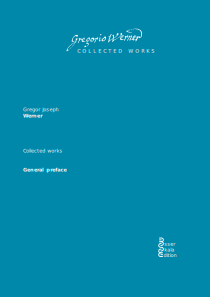
\includepdf{cover_general_preface.pdf}
\pagenumbering{arabic}
\setcounter{page}{1}

\tableofcontents

\chapter{General preface}

\textit{Gregor Joseph Werner: Collected works} (GJW:CW) is an edition project that will make Werner’s music available in modern editions. Simultaneously, it provides the source code used for typesetting the scores, thereby establishing a digital corpus of Werner’s works that follows FAIR principles.

For more information, we refer the reader to our thematic catalogue of Werner’s works, which is currently under development (\href{https://gregor-joseph-werner.at}{https://gregor-joseph-werner.at}). WerW numbers are cited from this catalogue.


\section{Editorial guidelines}

In general, GJW:CW follows the \href{https://edition.esser-skala.at/about/editorial-guidelines/}{editorial guidelines} for the Edition Esser-Skala.


\section{Acknowledgements}

Assistance of the following people and institutions is gratefully acknowledged:
Thomas Dolezal (Dommusikarchiv Eisenstadt – A-Ed),
Heidrun Boshof (Diözesanarchiv Graz-Seckau – A-Gdab),
Ute-Eva Thiem (Benediktinerabtei Stift Göttweig, Musikarchiv – A-GÖ),
H. Ulrich Mauterer CanReg (Stift Herzogenburg, Musikarchiv – A-H),
P. Roman Nägele OCist (Stift Heiligenkreuz im Wienerwald, Musikarchiv – A-HE),
Martin Haltrich and Ulrike Wagner (Stift Klosterneuburg, Musikarchiv – A-KN),
P. Altman Pötsch OSB (Benediktinerstift Kremsmünster, Regenterei und Musikarchiv – A-KR),
Peter Deinhammer (Benediktinerstift Lambach, Musikarchiv – A-LA),
P. Michael Eppenschwandtner OSB (Benediktinerabtei Michaelbeuern, Musikarchiv – A-MB),
P. Nikolaus Thiel OCist (Stift Schlierbach, Musikarchiv – A–SB),
Eva Neumayr (Archiv der Erzdiözese Salzburg, Musiksammlung – A-Sd),
P. Florian Ehebruster OSB (Benediktinerstift Seitenstetten, Musikarchiv – A-SEI),
Johannes Prominczel, Spiridoula Katsarou, and Günther Faimann (Archiv der Gesellschaft der Musikfreunde in Wien – A-Wgm),
P. Martin Gyöngyös OP (Bibliothek der Dominikanerprovinz Wien – A-Wdp),
Ikarus Kaiser (Stift Wilhering, Musikarchiv – A-WIL),
Michael Sipka (Erzbischöfliches Priesterseminar – A-Wps),
Stefan Engl and Ute Schmidthaler (Wienbibliothek im Rathaus, Musiksammlung – A-Wst),
Andreas Gamerith (Stift Zwettl, Stiftsbibliothek – A-Z),
Ilse Beel (Koninklijk Conservatorium Brussel, Bibliotheek – B-Bc),
Lenka Kluková (Archiv Pražského hradu, Praha – CZ-Pak),
Maria Šťastná (Knihovna Národního muzea, Praha – CZ-Pn and CZ-Pnm),
Gertraud Gaukesbrink (Santini-Bibliothek, Münster – D-MÜs),
Christoph Hauser (Benediktinerabtei Ottobeuren, Bibliothek – D-OB),
Gábor Nemes and Róbert Oláh (Székesegyházi Kottatár, Győr – H-Gk),
Zita Grócz (Érseki Könyvtár, Kalocsa – H-K),
Zoltán Damásdi (Pécsi Egyházmegye, Pécsi Püspöki Levéltár, Székesegyházi Kottatár – H-P),
Bálasz Karlinszky (Székesegyházi Kottatár, Veszprém – H-VEs),
Michiko Morita (Musashino Ongaku Daigaku, Tokyo – J-Tma),
Алла Алексеевна Семенюк (Российская государственная библиотека – RUS-Mrg),
Kristína Hrivňáková (Archív mesta Bratislavy – SK-BRm),
Dave McMullin (New York Public Library for the Performing Arts, Music Division – US-NYp),
Elisabeth Hilscher (Austrian Academy of Sciences),
James I. Armstrong (William and Mary, VA, USA),
Sieglinde Größinger-Potzmann,
Kornraset Narkmun,
Matthias J. Pernerstorfer (Don Juan Archiv Wien),
Jana Perutková (Masarykova Univerzita),
Klaus Petermayr (Oberösterreichisches Landesmuseum, Musiksammlung),
Natalie Stadler and Nils Grosch (Universität Salzburg),
as well as the staff of
the Österreichische Nationalbibliothek, Musiksammlung, Wien (A-Wn),
the Staatsbibliothek zu Berlin - Preußischer Kulturbesitz, Musikabteilung (D-B),
the Sächsische Landesbibliothek - Staats- und Universitätsbibliothek, Dresden (D-Dl),
the Universitäts- und Landesbibliothek Darmstadt, Musikabteilung (D-DS),
the Országos Széchényi Könyvtár, Budapest (H-Bn),
the Duke University Libraries, Music Library, Durham, NC (US-DMu),
the Zentral- und Hochschulbibliothek Luzern (CH-Lz),
and the Haydneum – Hungarian Centre for Early Music.


\clearpage
\markdownInput{../CHANGELOG.md}

\end{document}
